
\section{Implementation}
\label{sec:impl}



\begin{table*}[t]
\centering
\begin{small}
\begin{tabular}{|c|c|c|}
\hline
\multicolumn{3}{|c|}{Event Conditions (each has a cookie, not shown)} \\
\hline
Condition &           Parameters  &                             Description\\
\hline
Knock  &               cookie,src\_IP, src\_port &                        A remote host is attempting to open a connection \\
Connected &            cookie,outcome  &                                  A locally initiated flow has finished connecting\\
Recv &                 cookie, mbuf\_ptr, mbuf\_len &                  A message buffer has been received\\
Sent &                 cookie, bytes\_sent, window\_size &          Packet transmission has completed and/or the window size has changed \\
Dead &                cookie, reason &                                    The flow has been closed or an error has occurred \\
\hline
\hline
\multicolumn{3}{|c|}{Batched System Calls (partial list)} \\
\hline
connect &            cookie, dst\_IP, dst\_port &            Open a connection\\
accept &               handle, cookie &                          Accept a connection\\
sendv &               handle, scatter\_gather\_array &      Transmits an array of addresses and lengths\\
recv\_done &          handle, bytes\_acked &                Advances the receive window and frees memory buffers\\
close &                 handle &                                      Closes a connection\\
\hline
\end{tabular}
\caption{\ix event conditions and batch system calls}
\label{tbl:api}
\end{small}
\end{table*}




We now describe the implementation of the \ix prototype.  We start
with an overview of the \ix kernel (\S\ref{sec:impl:kernel}), describe
the environment surrounding \ix (\S\ref{sec:impl:env}), and how \ix is
implemented as a coherency-free kernel (\S\ref{sec:impl:cohfree}).


%the benefits of having \ix run as a guest
%operating system (\S\ref{sec:impl:guest}), its native API at the
%kernel/user boundary (\S\ref{sec:impl:api}), the implementation of the
%networking stack (\S\ref{sec:impl:stack}), the implications on
%congestion management and flow control (\S\ref{sec:impl:net}), the
%benefits and consequences of coherence-free execution
%(\S\ref{sec:impl:cohfree}), and finally our approach to compatibility
%(\S\ref{sec:impl:libix}).


\subsection{The \ix Kernel}
\label{sec:impl:kernel}



The \ix kernel consists of 37 KSLOC (according to SLOCcount
2.26~\cite{url:sloccount}), of which 43\% is derived from the Intel
device driver, 23\% from the lwIP TCP stack, and 16\% from the Dune
library and sandboxing module.  All three existing code bases are
highly modified for the purpose; the rest is approximately 7KSLOC of
new code.  The \ix kernel merges two distinct functions, as it is both
an operating system and a dataplane.

\myparagraph{Control flow:} \ix is an single address-space OS that can launch and run a single
legacy, multi-threaded POSIX application. \ix supports two distinct
thread types within the shared, userlevel address space: (i)
\emph{elastic threads} which interact with the \ix kernel to initiate
and consume network I/O and (ii) \emph{background threads} who can
issue arbitrary POSIX calls, including ones with blocking conditions.
Elastic threads interact essentially interact with the kernel through
three asynchronous, non-blocking mechanisms: they consume \emph{event
  conditions} generated by the kernel, have a direct, but safe, access
to message buffers \emph{mbuf}) containing incoming networking
payload, and can issue \emph{batched systems calls} to the kernel.

\myparagraph{Run to completion:} 
Fig.~\ref{fig:queues-cores} illustrates the run-to-completion model of the
dataplane for a multi-NIC, multi-queue and multi-core configuration.
Hardware NIC queues are assigned to elastic threads, which run
independently.  The elastic thread (i) polls the receive queues of the
NIC to dequeue all newly received packets into an in-memory queue, and
post fresh descriptors; 
 (ii) processes a bounded number of packets
through the incoming networking stack, thereby generating event
conditions; (iii) passes control to the user-space applications, which
consumes all event conditions, and in return responds with a batch of
system calls; (iv) upon return of control from user-space, \ix
processes all system calls, and in particular the ones that direct
outgoing networking traffic; (v) run all kernel timers, in particular
to ensure compliant TCP behavior; (vi) ensures that all outgoing
Ethernet frames can be put into NIC TX descriptor rings.

\myparagraph{API:} 
Table~\ref{tbl:api} enumerates the most important event conditions and
batched system calls of \ix.  Unlike a traditional OS with POSIX
sockets, \ix directly (but safely) exposes message buffers to
applications for a zero-copy access to the incoming payload.
Applications can then hold on to message buffers and release them via
a batched system call.  \ix also differs in directly exposing flow
control conditions to application: the \texttt{sendv} batched system
call does not synchronously return the number of bytes sent; instead,
the \texttt{Recv} event condition provides that information in a
subsequent step.  

\myparagraph{Security model:} Applications are
untrusted and can not access kernel memory (except for message
buffers) or network hardware.  No sequence of batched system calls or
other user-level actions can be used to violate correct adherence to
TCP and other network specifications.  Furthermore, the dataplane can
be used to enforce network security policies (e.g., iptables or Amazon
Security Groups) or to implement the network virtualization functions
typically done in a hypervisor~\cite{nsdi:nsx}.  However, and as a
consequence of the zero-copy model, applications have read-only access
to entire message buffers, including protocol headers.  Flow control
and receive buffer management is, however, entrusted to the user
runtime. Applications could misuse this ability to use up all of their
available memory, but it would only harm its own \ix instance.

\subsection{The environment}
\label{sec:impl:env}

\begin{figure}
\begin{centering}
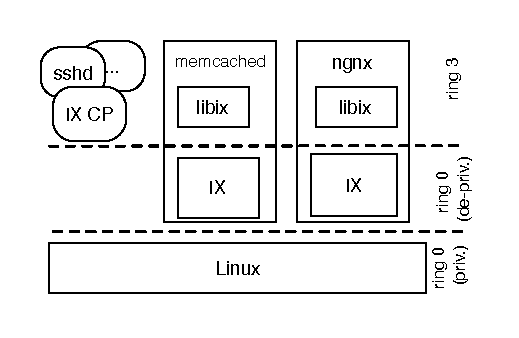
\includegraphics{figs/cp-dp.eps}
\vspace*{-3em}\caption{Protection and separation in \ix.}\vspace*{-1em}
\label{fig:cp-dp}
\end{centering}
\end{figure}



Fig.~\ref{fig:cp-dp} illustrates the environment that surrounds the
\ix kernel.  We rely on VT-x hardware
virtualization~\cite{DBLP:journals/computer/UhligNRSMABKLS05} to run
\ix as a guest operating system using Dune~\cite{belay2012dune}. Dune
itself runs as part of a Linux host and allows untrusted host
processes (in our case \ix) to securely access de-privileged hardware
functions.

\myparagraph{Separation and protection of control and data plane:}
Each \ix instance and its applications runs as a distinct Dune process
while control plane functions, including the control and monitoring of
dataplane, is performed by scripts and daemons of the host
environments.  This provides protection between control and
dataplanes. Within each dataplane, \ix further protects itself from
the untrusted application through virtual memory and by running it at
userlevel.

\myparagraph{Application compatibility:} We extended the Dune
sandboxing mechanisms to support the initial load of multi-threaded
applications into the userlevel address space, to launch both elastic
and background threads.  Although elastic threads could directly use
the native API of Table~\ref{tbl:api}, this would require a
substantial effort; the userlevel library therefore also includes a
compatibility mechanism that exposes the near-identical API as
\texttt{libevent}.  Both elastic and background threads can also issue arbitrary POSIX system
calls; those are merely intermediated by \ix, and handled by the
underlying OS.  Elastic threads are expected to \emph{not} issue blocking
system because of the adverse impact on network behavior and
performance.

\myparagraph{Resource management:}
We rely on Linux's ability to allocate resources at a coarse grain to
demanding applications, in our case the Dune processes.  For example,
core allocation can be precisely controlled through real-time
priorities and \texttt{cpumasks}; memory can be allocated in 2MB and
1GB chunks from specified NUMA nodes; PCI devices, virtual functions,
and NIC hardware queues alike can be assigned to specified \ix
kernels, etc.  This explicitly favors scalability and performance by
multiplexing resources in space among the various dataplanes, but not
in time at a fine granularity.  For example, elastic threads are scheduled exclusively onto a CPU
allocation is explicitly revoked, using a protocol similar to the one
used in Exokernels~\cite{DBLP:conf/sosp/EnglerKO95}.  

\myparagraph{Elasticity policies:}
In contrast to the mechanisms, which are generic, different policies
can be envisioned to meet different use cases and optimization
functions.  If neither energy proportionality or server consolidation
is of any concern, the control plane can obviously launch a single
dataplane instance configured with the maximal available physical
resources.  In more realistic scenarios, the dataplane is
``right-sized'' to meet its service-level agreements with minimal
resource allocations.  The control plane can further dynamically add
or revoke CPUs from a dataplane instances, e.g., when the dataplane
signals some sustained congestion or violation of its service-level
agreements, or conversely when the allocated CPU resources are
underutilized.

\subsection{Coherency-free Execution}
\label{sec:impl:cohfree}

The \ix kernel implements a \emph{coherency-free} execution model:
although the elastic threads share the same address space, there is no
communication, synchronization, or cache-coherency traffic between the
elastic threads during common case operations.  This is a stronger
requirement than lock-free synchronization, which requires expensive
atomic instructions~\cite{DBLP:conf/sosp/DavidGT13}, even when a single thread uses a
particular lock in the normal case.  This was made possible because of
conscious design and implementation decisions, including one with an
important tradeoff.

\myparagraph{A commutative API:} According to the commutativity rule,
system call implementations can only be coherence-free if the API
itself is commutative~\cite{DBLP:conf/sosp/ClementsKZMK13}.  The \ix
API is commutative: events are processed independently on each elastic
thread; cookies identify flows but cannot be exchanged between
threads, and there is no file descriptor namespace.


\myparagraph{Memory management:} Each elastic thread manages its own
memory pools, hardware queues, event condition queue, and batched
system call queue; no synchronization is required to access any of
them.

\myparagraph{Flow-consistent hashing:} \ix relies on flow-consistent
hashing by the NIC hardeware to ensure that each elastic thread
operates on a disjoint subset of the TCP flows.  The coherency-free
implementation for accepted flows naturally follows the hardware's
decision.  The solution is more complex in the reverse: for outbound
connections, \ix selects the source ephemeral port based on the
requesting elastic thread. Since the Toeplitz hash function cannot be
reversed, \ix simply probes the ephemeral range and computes the
Toepliz hash until a match is found.  Consequently, communication
between an \ix client and a server may required up to one flow per
elastic thread.  As a side effect of the implementation, ephemeral
source port no longer form namespaces, which allows an \ix client to
support millions of outgoing connections.

\myparagraph{Arrays vs. bounded buffers:}
The implementation of event conditions and batched system calls
benefits directly from the explicit, cooperative control flow
transfers between \ix and the application.  Since there is no concurrent
execution by producer and consumer, event conditions and batched
system calls are implemented as arrays without relying on lock-free
synchronization primitives based on atomics. 


\myparagraph{Use RCU locks when necessary:}
\ix does have a small number of shared structures, including some that
require synchronization on updates.  For example, the ARP table is
shared by all elastic threads and protected by RCU
locks~\cite{mckenney1998read}, which means that reads are
coherency-free.  Updates, which are rare, are not.

